\documentclass[3p,review,times,sort&compress]{elsarticle}

\usepackage[utf8]{inputenc}
\usepackage{amsmath}
\usepackage{amssymb}
\usepackage{amsopn}
\usepackage{mathtools}
\usepackage{bm}
\usepackage{textcomp}
\usepackage{gensymb}
\usepackage{chemformula}
\usepackage{siunitx}
\sisetup{detect-all}
\DeclareSIUnit{\atpercent}{at.\%}
\DeclareSIUnit{\angstrom}{\protect \text {Å}}
\usepackage{graphicx}
\graphicspath{{./figs/}}
\usepackage[table,dvipsnames]{xcolor}
\definecolor{HeaderLine}{RGB}{0, 131, 162}
\usepackage{booktabs}
\usepackage{multirow}
\usepackage{array}
\usepackage{tabularx}
\usepackage{float}
\usepackage{subcaption}
\usepackage{geometry}
%\geometry{letterpaper,left=0.89in,right=0.89in, top=1in, bottom=1in} % Change page size
\usepackage[ruled,vlined]{algorithm2e}
\usepackage{dirtytalk}
\usepackage{cuted}
\usepackage[
  breaklinks=true,
  plainpages=false,
  hypertexnames=false,
  pdfpagelabels=true
]{hyperref}
\hypersetup{hidelinks}
\usepackage{cleveref}
\usepackage{xcolor}
%\usepackage{lineno}
%\modulolinenumbers[5]

\newcommand{\etal}{\textit{et al.~}}
\newcommand{\dogu}[1]{\textcolor{red}{\textit{Doğu}: #1}}

% \renewcommand{\dogu}{}

%\journal{Acta Materialia}

\makeatletter
\def\ps@pprintTitle{%
 \let\@oddhead\@empty
 \let\@evenhead\@empty
 \def\@oddfoot{}%
 \let\@evenfoot\@oddfoot}
\makeatother

\begin{document}

\sloppy

\begin{frontmatter}

\title{Design of Spinodal Microstructures in High-Dimensional Composition Spaces via Analytic Derivatives of CALPHAD Model Predictions}

\author[1]{Courtney Kunselman\corref{cor1}}
\ead{cjkunselman18@tamu.edu}
\author[1]{Do\u{g}uhan Sar\i{}t\"urk}
\author[1]{Siya Zhu}
\author[1]{Vahid Attari}
\author[1,2,3]{Raymundo Arr\'{o}yave}

\cortext[cor1]{Corresponding author}

\affiliation[1]{organization={Department of Materials Science and Engineering, Texas A\&M University},
                city={College Station},
                postcode={77843}, 
                state={TX},
                country={USA}}

\affiliation[2]{organization={J. Mike Walker '66 Department of Mechanical Engineering, Texas A\&M University},
                city={College Station},
                postcode={77843}, 
                state={TX},
                country={USA}}

\affiliation[3]{organization={Wm Michael Barnes '64 Department of Industrial and Systems Engineering, Texas A\&M University},
                city={College Station},
                postcode={77843}, 
                state={TX},
                country={USA}}

\begin{abstract}    
   
\end{abstract}

\begin{keyword}

\end{keyword}

\end{frontmatter}

% \linenumbers

\section{Introduction}

Spinodal decomposition is a phase separation process characterized by barrierless uphill diffusion resulting in a bicontinuous microstructure morphology with periodic oscillations in composition. Since properties arise from structure, it is important to identify regions of conditions space which may be unstable to composition fluctuations and susceptible to spontaneous phase separation when designing alloys. In some cases, spinodal decomposition is undesirable and can lead to significant hardening and embrittlement of single-phase ductile alloys \cite{wang2023spinodal} or provide a a pathway for the formation of brittle, deleterious phases \cite{dasari2023crystallographic}. On the other hand, spinodal and spinodal-assisted microstructures have recently been leveraged to overcome the strength-ductility tradeoff \cite{an2021spinodal,lee2025spinodal,zhang2022refinement}, tailor magnetic properties \cite{rao2021beyond,dong2024cooperative}, and improve thermoelectric performance \cite{duan2025spinodal}. 

Regardless of whether the designer is looking to exploit or avoid spinodal decomposition, such a region must first be located within a design space that is often high-dimensional. Because exhaustive experimental characterization of these large design spaces is infeasible, computational modeling approaches which can predict microstructure stability are essential for the efficient identification of spinodal regions. Recent work to this end includes high-throughput \textit{ab initio} calculations coupled with cluster expansion to construct CALPHAD-style Gibbs energy models \cite{usanmaz2016first} and a novel procedure not requiring any functional form of the free energy in which the spinodal decomposition process is modeled as a nucleation event infinitesimally close to the spinodal boundary \cite{divilov2024priori}. While these approaches do not require any empirical data and were well-validated with experiments, they were only demonstrated on binary systems. Showing promise for spinodal design in high-dimensional composition spaces, Koneru, Kadirvel, and Wang recently developed a CALPHAD-based high-throughput microstructure stability predictive framework specifically for the multi-principal element alloy (MPEA) or high entropy alloy (HEA) design problem \cite{koneru2022high,kadirvel2022exploration}. This framework, now implemented in Pandat \cite{cao2009pandat}, facilitates gauge-invariant prediction and visualization of summaries of Gibbs energy surface geometry such as eigenvalues and eigenvectors of the Gibbs energy Hessian, spinodal temperatures, and initial composition fluctuations. 


In this work, we start with the framework of Koneru, Kadirvel, and Wang as a foundation and demonstrate a few key extensions. First, rather than using numerical derivative approximations which can become computationally expensive as the number of components gets large, we employ the recently formalized Jansson derivative method to calculate analytic Gibbs energy Hessians in a robust and efficient manner \cite{kunselman2024analytically}. Second, instead of relying on access to commercial databases which may not contain models for all alloy systems of interest, we use the recently developed PhaseForge package \cite{sariturk_2025_15730911} to automatically construct multicomponent CALPHAD models from machine learning-based interatomic potentials (MLIP). Third, we include an estimate for the elastic energy contributions due to coherency strains which penalize phase separation and effectively shrink the miscibility gap and spinodal region. Fourth, instead of using a collection of constant core component (a type of pseudoternary) diagrams to visualize results, we employ affine projections \cite{vela2025visualizing} to summarize high-dimensional data on a single two-dimensional plot. 

Lastly, the entire workflow is packaged in an open-source tool available through the MaterialsFramework interface \cite{sariturk_2025_15731044}. Through this framework, modelers have whitebox access to the CALPHAD model, and as demonstrated in \cite{kunselman2025construction}, they can further refine parameters to any available computational or experimental data through ESPEI \cite{bocklund2019espei}. The remainder of this work will dive into the theory and methodology of determining microstructure stability from the Gibbs energy description of a phase and then demonstrate our framework to investigate the stability of the BCC phase in the Hf-Nb-Ti-V system.

\section{Theory}
\subsection{Developing Gibbs Energy Models From Universal Potentials}

The stability analysis described in the following section requires a molar Gibbs energy description of the solid solution phase of interest as a function of composition and temperature. Classical CALPHAD databases are resource-intensive to develop and may not exist for all alloy systems of interest. To overcome this limitation, we employ the PhaseForge package \cite{sariturk_2025_15730911}, which automates the construction of CALPHAD-compatible Gibbs energy models from MLIPs as described in \cite{zhu2025accelerating,zhu2025machine}. This approach replaces computationally expensive density functional theory (DFT) calculations with MLIP evaluations that are several orders of magnitude faster while maintaining thermodynamic accuracy.

The approach is built on the use of special quasirandom structures (SQS) \cite{zunger1990special} to represent disordered solid solutions in a periodic cell. An SQS is a periodic supercell whose short-range order parameters match those of a perfectly random alloy up to a pre-determined neighbor range, enabling the disordered state to be represented without requiring large supercells.

Following the compound energy formalism (CEF) as implemented in the Alloy Theoretic Automated Toolkit (ATAT) \cite{van2002alloy}, the molar Gibbs energy of solution phase $\beta$ with site fractions $\boldsymbol{y}$ at temperature $T$ is given by

\begin{equation}\label{eq:gibbs_cef}
    G^\beta_m(\boldsymbol{y}, T) = \left(G^\beta_{\mathrm{calc,nc}}(\boldsymbol{y}, T) - \sum_i x_i\, G^{\alpha_i}_{\mathrm{calc,nc}}(T)\right) + \sum_i x_i\, G^{\alpha_i}_{\mathrm{SGTE}}(T) - T S_{\mathrm{id}}(\boldsymbol{y}),
\end{equation}

where $G^\beta_{\mathrm{calc,nc}}$ is the Gibbs energy of phase $\beta$ computed from MLIP total energies without any configurational entropy contribution, $G^{\alpha_i}_{\mathrm{calc,nc}}$ is the corresponding quantity for pre component $i$ in its reference crystal structure $\alpha_i$, $G^{\alpha_i}_{\mathrm{SGTE}}$ is the unary Gibbs energy of component $i$ taken from the Scientific Group Thermodata Europe (SGTE) database \cite{dinsdale1991sgte}, $x_i$ is the mole fraction component $i$, and $S_{\mathrm{id}}(\boldsymbol{y})$ is the ideal configurational entropy. For a single-sublattice solution phase, the ideal configurational entropy reduces to

\begin{equation}\label{eq:conf_entropy}
    S_{\mathrm{id}}(\boldsymbol{y}) = -R\sum_i x_i\ln x_i,
\end{equation}

where $R$ is the ideal gas constant.

For each SQS supercell, the quantity $G^\beta_{\mathrm{calc,nc}}$ at \SI{0}{\kelvin} is taken directly from the MLIP-relaxed potential energy per atom. Structural relaxations are performed through the MaterialsFramework calculator interface \cite{sariturk_2025_15731044} with a force convergence criterion of $f_{\mathrm{max}} < \SI{0.001}{\electronvolt/\angstrom}$. For the BCC\_A2 phase in the \ch{Hf-Nb-Ti-V} system, the compositional dependence of the mixing energy is captured sufficiently by static formation energies, and thermal contributions are accounted for through the SGTE unary data.

Once formation energies have been computed for SQS supercells spanning the composition space of each phase, the composition-dependent mixing contribution embedded in $G^\beta_{\mathrm{calc,nc}}$ is parameterized using a Redlich-Kister polynomial expansion. For a binary \ch{A-B} subsystem, the excess Gibbs energy is expressed as

\begin{equation}\label{eq:rk}
    G^\beta_{m,\mathrm{xs}} = x_A x_B \sum_{\nu=0}^{k} L^{(\nu)}_{A,B}\,(x_A - x_B)^\nu,
\end{equation}

where $L^{(\nu)}_{A,B}$ are the $\nu$-th order binary interaction parameters determined by least-squares fitting to the MLIP-computed formation energies. Temperature-independent interaction parameters are assumed throughout. Higher-order ternary and quaternary interactions are incorporated analogously and are extracted by fitting to SQS energies at compositions spanning the multicomponent space.

The fitted interaction parameters are assembled into a thermodynamic database (TDB) file compatible with PyCalphad \cite{otis2017pycalphad}. The resulting TDB for the BCC\_A2 phase in the \ch{Hf-Nb-Ti-V} system serves as the thermodynamic input for the stability analysis described below.

\subsection{Determining Stability From the Gibbs Energy Hessian}

Gibbs first introduced the concept of a thermodynamic stability limit, or spinodal, by considering composition fluctuations leading to continuous changes in fluid phases \cite{gibbs1878equilibrium}. He determined that the limit of stability for such a phase relative to these fluctuations occurs where the derivatives of the chemical potential of each component with respect to the density of its corresponding component are equal to zero. That is, a system stable to all composition fluctuations experiences positive changes in all of its chemical potentials when the content of the corresponding component is increased. As Cahn explains in \cite{cahn1961spinodal}, for binary system $A-B$ where $B$ is the dependent component, this limit of stability simplifies to the well-known expression

\begin{equation}\label{second_der_G}
    \frac{d^2G^\alpha_m}{dx^2_A}=0,
\end{equation}

\noindent where $G^\alpha_m$ is the molar Gibbs energy for phase $\alpha$ and $x_A$ is the composition of component $A$. 

Following Gibbs and Cahn, the pioneering work of de Fontaine rigorously derived the conditions for stability for solid phases in multicomponent systems by including coherency stress contributions to the free energy in both continuum \cite{de1967computer} and microscopic \cite{de1972analysis} contexts. In recent works, Kadirvel \etal provide an elegant condensed proof of these conditions using the continuum formulation \cite{kadirvel2022exploration}, and Morral and Chen apply de Fontaine's findings to comprehensibly extend Gibbs' work to the solid phase, multicomponent system context. We summarize their combined insight below.

Consider solid solution phase $\alpha$, an $n$-component phase with composition $\boldsymbol{x}$ for which we define the $n$-th component as the dependent composition variable. Let $\boldsymbol{\Delta}$ be a local arbitrary composition fluctuation in phase $\alpha$ defined for all independent composition variables. To maintain mass balance, a local composition fluctuation of $-\boldsymbol{\Delta}$ must also occur for an equivalent amount of the system. The molar Gibbs energy change of the portion of phase $\alpha$ affected by this composition fluctuation is given by

\begin{equation}\label{eq:energy_change}
\Delta G^\alpha_m = \frac{1}{2}G^\alpha_m(\boldsymbol{x}+\boldsymbol{\Delta}) + \frac{1}{2}G^\alpha_m(\boldsymbol{x}-\boldsymbol{\Delta}) -G^\alpha_m(\boldsymbol{x}).
\end{equation}

\noindent Using a second order Taylor series expanded around $\boldsymbol{x}$, we can approximate $G^\alpha_m(\boldsymbol{x}+\boldsymbol{\Delta})$ as 

\begin{equation}\label{eq:Taylor_1}
    G^\alpha_m(\boldsymbol{x}+\boldsymbol{\Delta})\approx G^\alpha_m(\boldsymbol{x}) + \sum_{i=1}^{n-1}\frac{\partial G^\alpha_m}{\partial x_i}\Delta_i+\frac{1}{2}\sum_{i=1}^{n-1}\sum_{j=1}^{n-1}\frac{\partial^2G^\alpha_m}{\partial x_i\partial x_j}\Delta_i\Delta_j
\end{equation}

\noindent and $G^\alpha_m(\boldsymbol{x}-\boldsymbol{\Delta})$ as

\begin{equation} \label{eq:Taylor_2}
    G^\alpha_m(\boldsymbol{x}-\boldsymbol{\Delta})\approx G^\alpha_m(\boldsymbol{x}) - \sum_{i=1}^{n-1}\frac{\partial G^\alpha_m}{\partial x_i}\Delta_i+\frac{1}{2}\sum_{i=1}^{n-1}\sum_{j=1}^{n-1}\frac{\partial^2G^\alpha_m}{\partial x_i\partial x_j}\Delta_i\Delta_j
\end{equation}

\noindent where all derivatives are evaluated at $\boldsymbol{x}$.

Substituting \Cref{eq:Taylor_1,eq:Taylor_2} into \Cref{eq:energy_change} gives

\begin{equation} \label{eq:Hessian}
\Delta G^\alpha_m = \sum_{i=1}^{n-1}\sum_{j=1}^{n-1}\frac{\partial^2G^\alpha_m}{\partial x_i\partial x_j}\Delta_i\Delta_j=\boldsymbol{\Delta}^TH\boldsymbol{\Delta}
\end{equation}

\noindent where $H$ is the Hessian of $G^\alpha_m$ with respect to the independent composition variables. Assuming that all entries of the Hessian are continuous throughout the composition domain, we can claim that $H$ is a symmetric matrix with real eigenvalues $\lambda_1,\hdots,\lambda_{n-1}$ and a corresponding set of eigenvectors $\boldsymbol{v}_1,\hdots,\boldsymbol{v}_{n-1}$ which form an orthonormal basis in the space defined by the independent composition variables. Thus, $\boldsymbol{\Delta}$ can be written as a linear combination of this basis:

\begin{equation} \label{eq:projection}
    \boldsymbol{\Delta} = \sum_{i=1}^{n-1} (\boldsymbol{\Delta}^T\boldsymbol{v}_i)\boldsymbol{v}_i.
\end{equation}

\noindent Substituting \Cref{eq:projection} into \Cref{eq:Hessian} and leveraging the relationship between eigenvalues and eigenvectors ($H\boldsymbol{v}_i=\lambda_i\boldsymbol{v}_i$) gives

\begin{equation}\label{eq:final_delta_G}
\begin{split}
    \Delta G^\alpha_m &= \left(\sum_{i=1}^{n-1}(\boldsymbol{\Delta}^T\boldsymbol{v}_i)\boldsymbol{v}_i\right)^TH\left(\sum_{i=1}^{n-1}(\boldsymbol{\Delta}^T\boldsymbol{v}_i)\boldsymbol{v}_i\right)\\&=\left(\sum_{i=1}^{n-1}(\boldsymbol{\Delta}^T\boldsymbol{v}_i)\boldsymbol{v}_i\right)^T\left(\sum_{i=1}^{n-1}(\boldsymbol{\Delta}^T\boldsymbol{v}_i)\lambda_i\boldsymbol{v}_i\right)=\sum_{i=1}^{n-1}\lambda_i(\boldsymbol{\Delta}^T\boldsymbol{v}_i)^2.
    \end{split}
\end{equation}

\noindent Thus, as \Cref{eq:final_delta_G} illustrates, such a composition fluctuation can only lower the Gibbs energy if at least one of the eigenvalues is negative, and a zero-valued eigenvalue represents the limit of stability, or the spinodal. If only one eigenvalue, say $\lambda_1$, is negative, the system is conditionally unstable to composition fluctuations in the direction of $\boldsymbol{v}_1$, or equivalently, with large values for the projection $\boldsymbol{\Delta}^T\boldsymbol{v}_1$. More negative eigenvalues lead to more directions for $\boldsymbol{\Delta}$ to be unstable, and $n-1$ negative eigenvalues imply that the solid solution is unstable to any $\boldsymbol{\Delta}$.

As Morral and Chen \cite{morral2021stability} and Kadirvel \etal \cite{kadirvel2022exploration} both report, these eigenvalues and eigenvectors are not gauge invariant. That is, $\lambda_1,\hdots,\lambda_{n-1}$ and $\boldsymbol{v}_1,\hdots,\boldsymbol{v}_{n-1}$ depend on the choice of the dependent component. This is due to a combination of the coordinate axes being geometrically non-orthogonal and the change in orientation of these axes with the variation of the dependent component. 

To address this issue, Kadirvel \etal \cite{kadirvel2022exploration} followed the approach of Singh \etal \cite{singh2015atomic} which involves a change of basis operation transforming $H$ from Gibbs simplex space to Cartesian space, performing the eigenanalysis in Cartesian space, and lastly transforming the resulting eigenvectors back to Gibbs space (the eigenvalues calculated in Cartesian space remain invariant under this final transformation). Singh \etal \cite{singh2015atomic} provide an iterative procedure for constructing such an $N$-dimensional linear transformation, and Kadirvel \etal \cite{kadirvel2022exploration} explicitly provide this matrix for systems with ten components or fewer. In this work, we adopt this approach in order to calculate and visually display the distribution of gauge-invariant eigenvalues. 

Lastly, for arbitrarily-complex phases modeled with internal degrees of freedom (or equivalently, for any phase with a Gibbs energy function that is multivalued in composition space), calculating the Gibbs energy Hessian requires differentiating the outputs of single-phase energy minimization calculations. These equilibrium calculations prescribe the composition of the phase (not the system) and determine the local minimum solution (which may be metastable) under this composition constraint. For phase $\alpha$ in ternary system A-B-C, it is well known that the first derivative of $G^\alpha_m$ with respect to $x_A$ can be written as a simple linear combination of chemical potentials

\begin{equation}\label{eq:first_derivative}
\frac{\partial G^\alpha_m}{\partial x_A}=\mu_A-\mu_C
\end{equation}

\noindent where $C$ is the dependent component. Thus, second order derivatives can be expressed as 

\begin{equation}\label{eq:second_derivatives}
    \frac{\partial^2G^\alpha_m}{\partial x_B\partial x_A} = \frac{\partial \mu_A}{\partial x_B} - \frac{\partial \mu_C}{\partial x_B},
\end{equation}

\noindent but calculation of \Cref{eq:second_derivatives} is less trivial. In this work, we employ the recently formalized Jansson derivative method \cite{kunselman2024analytically}, an adjoint-like technique for calculating analytic derivatives of thermodynamic properties at equilibrium with respect to CALPHAD model equilibrium calculations, to efficiently calculate the derivatives of the chemical potentials in \Cref{eq:second_derivatives} rather than relying on numerical approximations. All Gibbs energy Hessians are computed using PyCalphad \cite{otis2017pycalphad} (development version commit a8de09f).

Using the procedure described above, we can employ Jansson derivatives to calculate the chemical Hessian and corresponding chemical spinodal from a CALPHAD Gibbs energy description of a solution phase. However, in many solid solutions, composition fluctuations can lead to significant elastic energy contributions due to coherency strains. These coherency strains penalize composition fluctuations and when their elastic energy contributions are added to the chemical Gibbs energy, the spinodal region shrinks. \textcolor{red}{Siya: We have to clarify that we assume the coherence is "biaxial" and the system is "infinite isotropic".}As Cahn shows in \cite{cahn1961spinodal}, for an infinite binary isotropic solid with an arbitrary composition fluctuation \textcolor{red}{Siya: I think the equation given by Cahn works only for infinitesimal coherent composition fluctuations instead of arbitrary or finite-amplitude composition fluctuations. He dropped the higher order terms in equation(2) and wrote "for small (c-c0)" above equation(7) in his paper.} , when coherency strains are considered the limit of stability given in \Cref{second_der_G} becomes

\begin{equation}
    \frac{d^2G^\alpha_m}{dx^2_A}+\frac{2\eta_A^2EV_m}{1-\nu}=0
\end{equation}

\noindent where $E$ is the modulus of elasticity, $V_m$ is the molar volume, $\nu$ is the Poisson ratio, and $\eta_A$ is the linear strain per unit difference in component $A$:

\begin{equation}
\eta_A=\frac{1}{a}\frac{\partial a}{\partial x_A}
\end{equation}

\noindent where $a$ is the lattice parameter. Extending to the multicomponent context \cite{de1973analysis}, entries of the coherent Hessian $H^{coh}$ are given by

\begin{equation}
    H^{coh}_{ab}=\frac{\partial^2G^\alpha_m}{\partial x_B\partial x_A}+\frac{2\eta_A\eta_BEV_m}{1-\nu}
\end{equation}

\noindent where $\frac{\partial^2G^\alpha_m}{\partial x_B\partial x_A}$ is the chemical contribution as calculated in \Cref{eq:second_derivatives}.

In this work, we employ the bond-based lattice parameter prediction model \textcolor{red}{Siya: why don't we use the lattice parameters from the relaxed SQS directly? Courtney: because we wanted an analytic model for the lattice parameter that we could easily differentiate to calculate eta.} developed by Tandoc \etal \cite{tandoc2025bond} to calculate $\boldsymbol{\eta}$ and $V_m$. Under this model, the average lattice parameter $\bar{a}$ for a solid solution BCC phase is given by

\begin{equation}\label{lattice_param}
    \bar{a}=\frac{2\bar{d}_{111}}{\sqrt{3}}
\end{equation}

\noindent where $\bar{d}_{111}$ is the average bond length along the $<111>$ close-packed direction. The average bond length is calculated through

\begin{equation}
    \bar{d}_{111}=\sum_i\sum_jx_ix_jd^{ij}_{111}
\end{equation}

\noindent where $d^{ij}_{111}$ is the first nearest neighbor (FNN) bond length for an $i-j$ pair along the $<111>$ close-packed direction, following the framework of Tandoc \etal \cite{tandoc2025bond}. Same-species bond lengths $d^{ii}_{111}$ are extracted from MLIP-relaxed pure BCC cells via $d^{ii}_{111} = a_i^{\text{BCC}}\sqrt{3}/2$, while cross-species lengths $d^{ij}_{111}$ ($i \neq j$) are obtained from MLIP-relaxed B2 (\ch{CsCl}-type) binary ordered cells via $d^{ij}_{111} = a_{ij}^{\text{B2}}\sqrt{3}/2$. All relaxations for bond length extraction are performed using the \texttt{BondLatticeParameter} tool within MaterialsFramework \cite{sariturk_2025_15731044} with the GRACE-2L-SMAX-OMAT-large universal MLIP. Using this model for BCC structures, the molar volume is then given by

\begin{equation}
V_m=\frac{\bar{a}^3N_A}{2}
\end{equation}

\noindent where $N_A$ is Avogadro's number. To calculate derivatives of the lattice parameter for $\eta$, a dependent component must be assigned which must remain consistent throughout the calculation of the coherent Hessian. Let $k$ be the index of the dependent component. Then

\begin{equation}
    x_k=1-\sum_{i\neq k}x_i,
\end{equation}

\noindent and

\begin{equation}\label{bond_length_dep}
\bar{d}_{111}= \sum_{i\neq k}\sum_{j\neq k}x_ix_jd^{ij}_{111} + \sum_{i\neq k} x_i(1-\sum_{j\neq k}x_j)d^{ik}_{111} + \sum_{i\neq k}(1-\sum_{j\neq k}x_j)x_id^{ki}_{111} + (1-\sum_{j\neq k}x_j)^2d^{kk}_{111}.
\end{equation}

\noindent Differentiating \Cref{bond_length_dep} with respect to independent composition variable $x_1$ gives

\begin{small}
\begin{equation}\label{bond_length_der_dep}
\begin{split}
\frac{\partial \bar{d}_{111}}{\partial x_1}&=\sum_{i\neq k}(x_id^{i1}_{111}+x_id^{1i}_{111})-\sum_{i\neq 1,k}(x_id^{ik}_{111}+x_id^{ki}_{111})+(1-2x_1-\sum_{i\neq 1,k}x_i)d^{1k}_{111}\\ & + (1-2x_1-\sum_{i\neq 1,k}x_i)d^{k1}_{111} - 2(1-\sum_{i\neq k} x_i)d^{kk}_{111}\\&
=2\left(\sum_{i\neq k}x_id^{i1}_{111} - \sum_{i\neq 1,k} x_id^{ik}_{111} + (x_k-x_1)d^{1k}_{111}-x_kd^{kk}_{111}\right).
\end{split}
\end{equation}
\end{small}

\noindent Differentiating \Cref{lattice_param} and plugging in the result from \Cref{bond_length_der_dep}, we have

\begin{equation}
\frac{\partial \bar{a}}{\partial x_1}=\frac{4}{\sqrt{3}}\left(\sum_{i\neq k}x_id^{i1}_{111} - \sum_{i\neq 1,k} x_id^{ik}_{111} + (x_k-x_1)d^{1k}_{111}-x_kd^{kk}_{111}\right).
\end{equation}

Lastly, the elastic constants $C_{11}$, $C_{12}$, and $C_{44}$ were computed for each composition of interest using the \texttt{CubicElasticConstantsAnalyzer} within the MaterialsFramework package \cite{sariturk_2025_15731044}. A $4\times4\times4$ BCC SQS supercell was first relaxed using the GRACE-2L-SMAX-OMAT-large universal MLIP with unconstrained cell shape to a force convergence of $f_{\mathrm{max}} < \SI{0.01}{\electronvolt/\angstrom}$. Three finite strain modes were then applied to the relaxed cell: a uniform volumetric distortion to extract the bulk modulus $B$, an orthorhombic distortion to isolate $C'=\left(C_{11}-C_{12}\right)/2$, and a monoclinic shear to determine $C_{44}$. Polycrystalline-averaged elastic properties were then obtained via the Voigt-Reuss-Hill (VRH) scheme, yielding the macroscopically isotropic Young's modulus $E$ and Poisson's ratio $\nu$. The biaxial modulus $M = E/\left(1-\nu\right)$ appearing in the coherent Heissian above was derived directly from these VRH averages. \textcolor{red}{Siya: Are the Young's moduli and Poisson's ratio assumed isotropic? The Cahn's model requires the isotropy. How does materialsframework deal with that? For bcc structure the isotropy is described as $A=\frac{2C_{44}}{C_{11}-C_{12}}$ and is isotropic when $A=1$. For Nb, given by "Elastic Constants of Niobium from 4.2 to 300K", K. Carroll, J. Appl. Phys., 1965., at 300K, the $C_{11}$ is $24.56\times 10^{11} dyn/cm^2$, the $C_{12}$ is $13.87\times 10^{11} dyn/cm^2$, and the $C_{44}$ is $2.930\times 10^{11} dyn/cm^2$, $A = 0.548$. The Young's moduli and Poisson ratio calculated based on the experimental data are:
} 

\begin{table}[htbp]
\centering
\color{red}
\caption{\textcolor{red}{Direction-dependent Young's modulus and Poisson's ratio of single-crystal Nb at 300 K, calculated from the experimental elastic constants
$C_{11}=245.6$ GPa, $C_{12}=138.7$ GPa, and $C_{44}=29.30$ GPa.}}
\label{tab:nb_directional_elasticity}
\begin{tabular}{cccc}
\hline
Loading direction & Transverse direction & $E$ (GPa) & $\nu$ \\
\hline
$[100]$ & $[010]$ & 145.5 & 0.361 \\
$[110]$ & $[1\bar{1}0]$ & 93.2 & 0.591 \\
$[110]$ & $[001]$ & 93.2 & 0.231 \\
$[111]$ & $[1\bar{1}0]$ & 83.2 & 0.420 \\
\hline
\end{tabular}
\end{table}
\textcolor{red}{How we decide the $E$ and $\nu$ in Equation 12?}

\subsection{Verifying Microstructure Instability with Phase Field Modeling} 

\clearpage
\section{Investigating Spinodal Decomposition in the Hf-Nb-Ti-V System}

The sections below apply the MLIP-informed pipeline---ORB potential energies, Jansson-based chemical potential derivatives, and a semi-implicit spectral Cahn--Hilliard solver---to the \ch{Hf-Nb-Ti-V} system.
We progress from binary to quaternary subsystems, demonstrating at each stage how thermodynamic driving forces, coherency strain, and numerical tractability jointly govern which compositions and temperatures are accessible to simulation.

Selecting a productive target composition requires meeting two criteria simultaneously.
The composition must be spinodally unstable ($\lambda_{\min} < 0$ for the Gibbs energy Hessian), and no individual element should exhibit a large positive diagonal Hessian entry $H_{ii} = \partial^2 G^\alpha_m / \partial x_i^2 \gg 0$ at the nominal composition.
Elements satisfying the latter condition are thermodynamically stable spectators: they do not drive decomposition, yet through the stability constraint on the semi-implicit spectral solver,
\begin{equation}
    \Delta t \;\leq\; \frac{C_{\rm s}\,\Delta x^{2}}{M\,H_{\max}},
    \label{eq:dt_stability}
\end{equation}
where $C_{\rm s} = 0.3$ is a safety factor, $\Delta x$ the grid spacing, $M$ the atomic mobility, and $H_{\max}$ the largest Hessian eigenvalue, they reduce the allowable time step by one to two orders of magnitude without contributing to any spinodal driving force (Supplementary Table~S1).
We address both criteria by studying the binary, ternary, and quaternary subsystems in sequence, selecting compositions and temperatures at which the spinodal is both thermodynamically strong and numerically tractable.

\subsection{Thermodynamic Stability Landscape}
\label{sec:stability_landscape}

The spinodal region of the BCC\textsubscript{A2} phase spans a wide but structured region of the Hf--Nb--Ti--V composition space whose extent and character change substantially with temperature.
Figure~\ref{fig:stability maps} shows affine projections of the number of negative eigenvalues of the chemical and coherent Gibbs energy Hessians at \qtylist{600;800;1000}{\kelvin}, computed at \SI{5}{\atpercent} sampling density in composition space.
Missing points represent convergence failures, most common at dilute compositions.
At \SI{600}{\kelvin}, coherent strain contributions most strongly suppress the chemical spinodal at compositions rich in Hf or V, and the region of two negative chemical eigenvalues vanishes entirely when coherency is included.
At \SI{800}{\kelvin}, the chemical Hessian predicts spinodal decomposition across nearly all compositions except those rich in Ti and Nb, while the coherent Hessian stabilizes solid solutions rich in both Hf and V.
At \SI{1000}{\kelvin}, coherent strain stabilizes all Ti- and V-rich compositions and the spinodal shrinks to a narrow Nb-rich band.

\begin{figure*}[!h]
        %\captionsetup[subfigure]{labelformat=empty}
        \centering
        \subfloat[(a)]{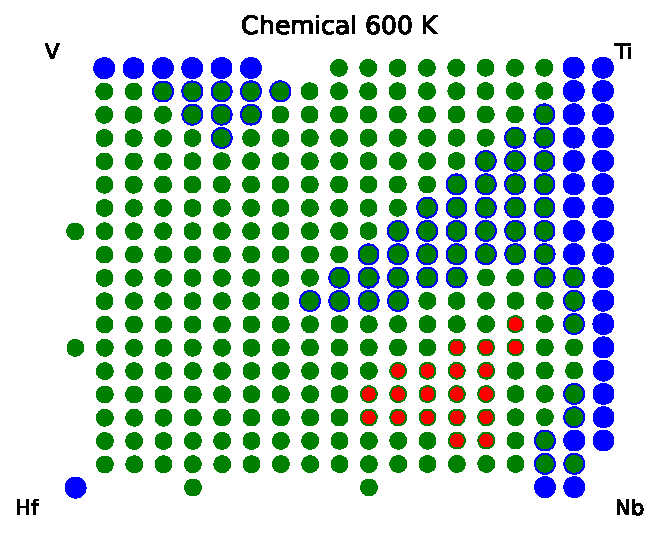
\includegraphics[width=.35\linewidth]{figs/chemical_600_diff_sizes.pdf}}\hspace{.3 in}
         \subfloat[(b)]{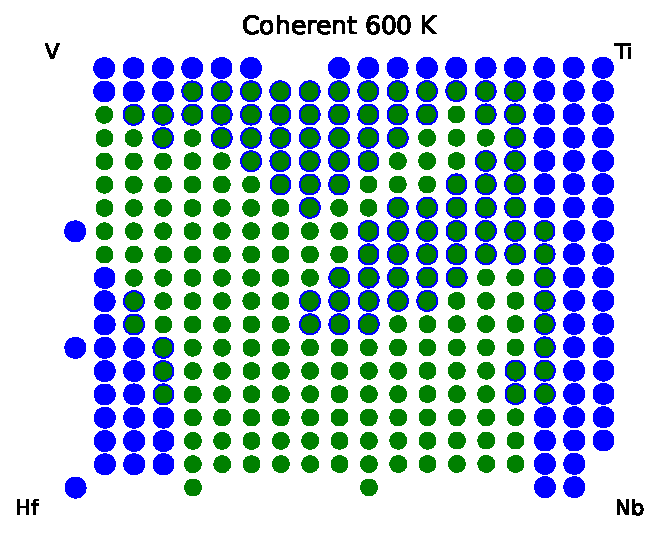
\includegraphics[width=.35\linewidth]{figs/coherent_600_diff_sizes.pdf}}\\
         \subfloat[(c)]{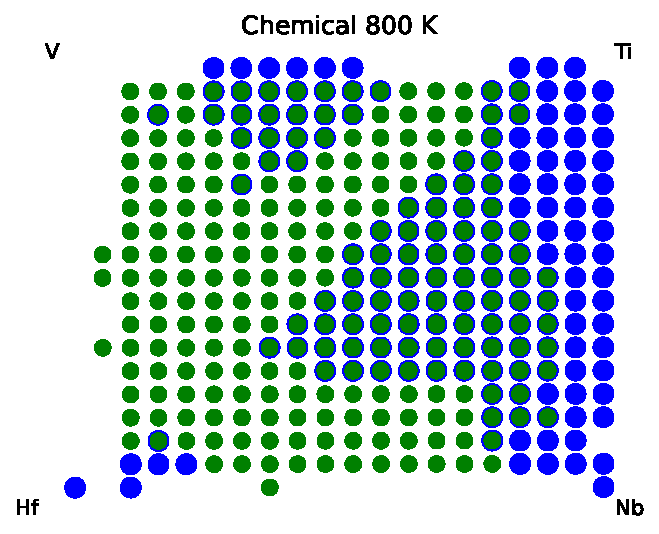
\includegraphics[width=.35\linewidth]{figs/chemical_800_diff_sizes.pdf}}\hspace{.3 in}
         \subfloat[(d)]{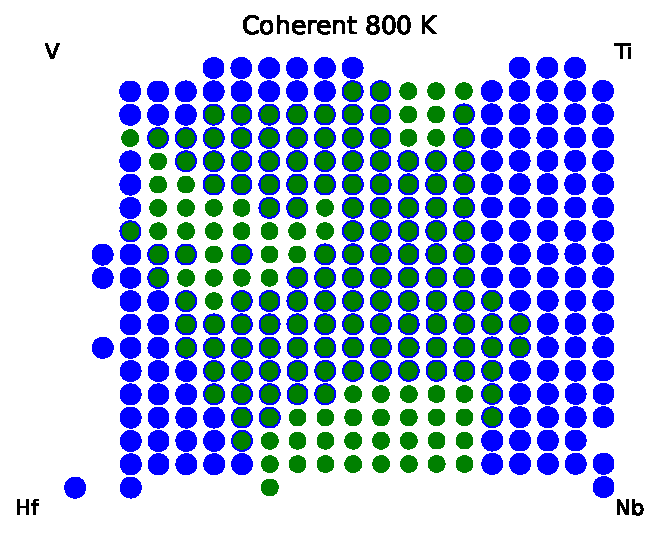
\includegraphics[width=.35\linewidth]{figs/coherent_800_diff_sizes.pdf}}\\
         \subfloat[(e)]{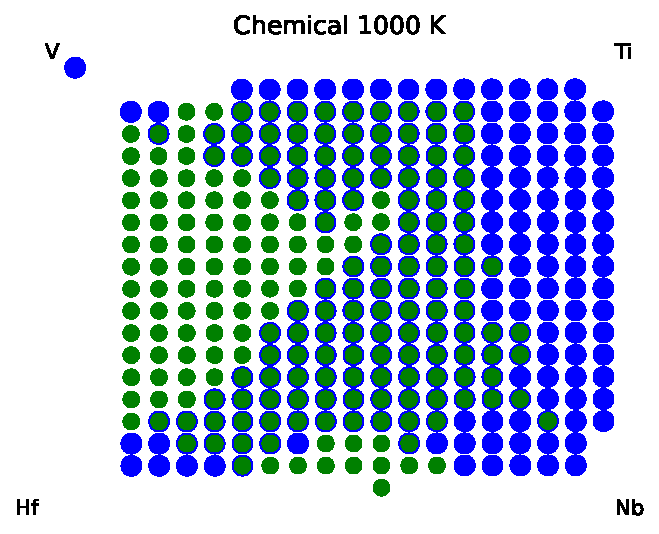
\includegraphics[width=.35\linewidth]{figs/chemical_1000_diff_sizes.pdf}}\hspace{.3 in}
         \subfloat[(f)]{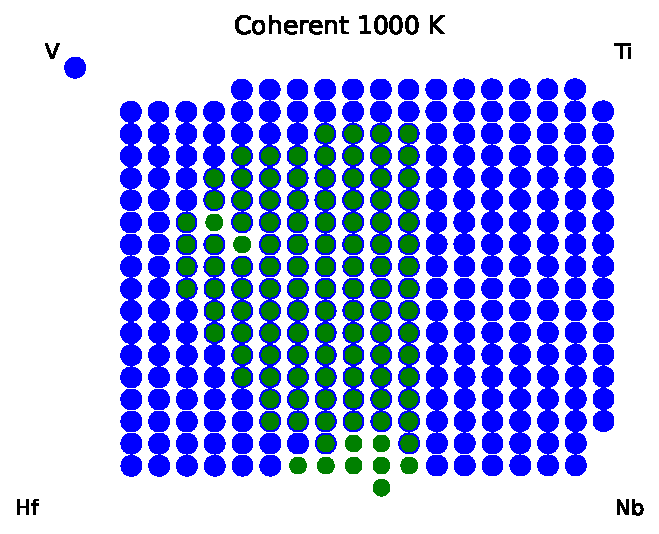
\includegraphics[width=.35\linewidth]{figs/coherent_1000_diff_sizes.pdf}}\\
         \subfloat[]
         {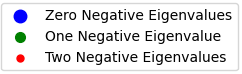
\includegraphics[width=.3\linewidth]{figs/legend.png}}
         \caption{Affine projection stability maps displaying the number of negative eigenvalues of the chemical and coherent Gibbs energy Hessian for BCC\textsubscript{A2} in the \ch{Hf-Nb-Ti-V} system at (a,b)~\SI{600}{\kelvin}, (c,d)~\SI{800}{\kelvin}, and (e,f)~\SI{1000}{\kelvin}.
         Left column: chemical Hessian; right column: coherent Hessian.
         Coherent strain suppresses the spinodal most strongly in Hf- and V-rich compositions across all temperatures.}
\label{fig:stability maps}
\end{figure*}

The mechanism by which coherency suppresses the Hf-rich spinodal is revealed by the first eigenvector of the chemical Hessian.
Figure~\ref{fig:eigenvector} shows the components of this vector for BCC \ch{Hf_{0.6}Nb_{0.1}Ti_{0.1}V_{0.2}} from \qtyrange{600}{1000}{\kelvin}, a composition at which the chemical Hessian is negative while all eigenvalues of the coherent Hessian are positive.
The unstable fluctuation mode corresponds to enrichment in Hf at the expense of V.
Since Hf and V have the largest atomic radius mismatch of the four constituents, this fluctuation mode incurs the greatest coherency penalty: adding the elastic contribution to the Gibbs energy reverses the sign of the local curvature and stabilizes the alloy against this mode throughout the temperature range shown.
The element pair that drives the chemical instability is self-suppressed by the strain energy it would generate.

\begin{figure*}[!h]
\centering
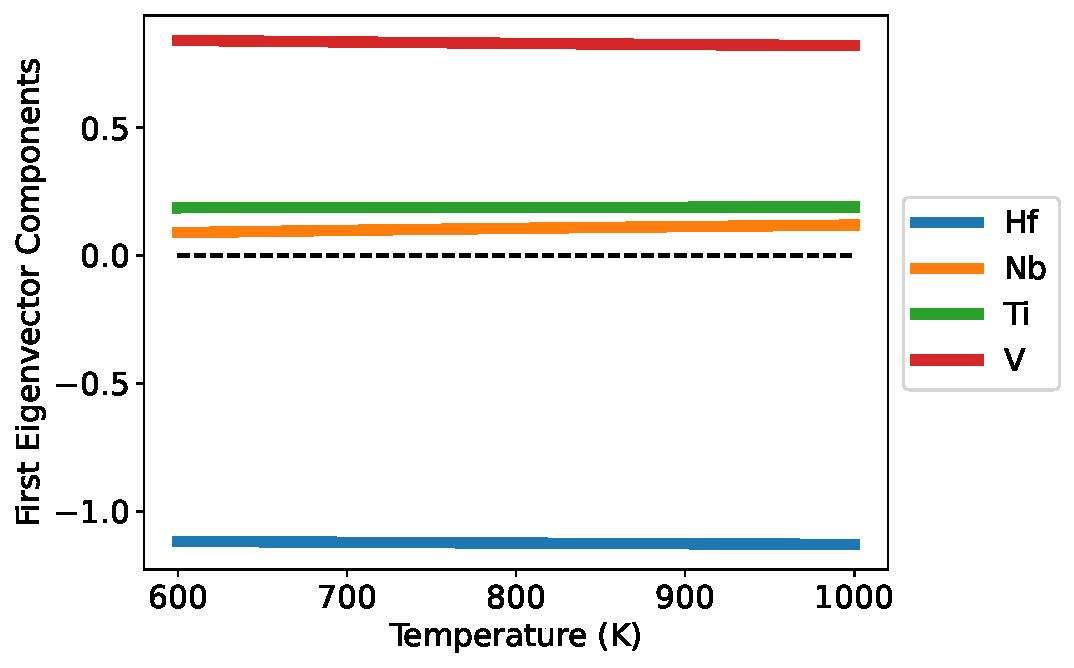
\includegraphics[width=\linewidth]{figs/eigenvector.pdf}
\caption{Components of the first gauge-invariant eigenvector of the chemical Hessian as a function of temperature for BCC \ch{Hf_{0.6}Nb_{0.1}Ti_{0.1}V_{0.2}}.
The dominant instability mode corresponds to Hf-enrichment at the expense of V; the large Hf--V atomic radius mismatch causes coherent strain to stabilize this mode at all temperatures shown, reversing the sign of the first eigenvalue from negative (chemical) to positive (coherent).}
\label{fig:eigenvector}
\end{figure*}

The temperature at which spinodal decomposition becomes accessible is composition-dependent and shifts substantially when coherency is included (Fig.~\ref{fig:eigenvalues}).
For the Ti- and Nb-rich composition \ch{Hf_{0.10}Nb_{0.40}Ti_{0.40}V_{0.10}}, the chemical and coherent spinodal temperatures are nearly identical, reflecting the small misfit penalty in dilute-Hf alloys.
For the equiatomic composition \ch{Hf_{0.25}Nb_{0.25}Ti_{0.25}V_{0.25}}, both Hessians become negative below ${\sim}\SI{800}{\kelvin}$, confirming that this alloy is coherently spinodal at \SI{500}{\celsius}, the temperature adopted for all phase-field simulations below.
For the Hf-rich composition \ch{Hf_{0.6}Nb_{0.1}Ti_{0.1}V_{0.2}}, the coherent Hessian remains positive at all temperatures shown, consistent with the eigenvector analysis above.

\begin{figure*}[!h]
        %\captionsetup[subfigure]{labelformat=empty}
        \centering
        \subfloat[(a)]{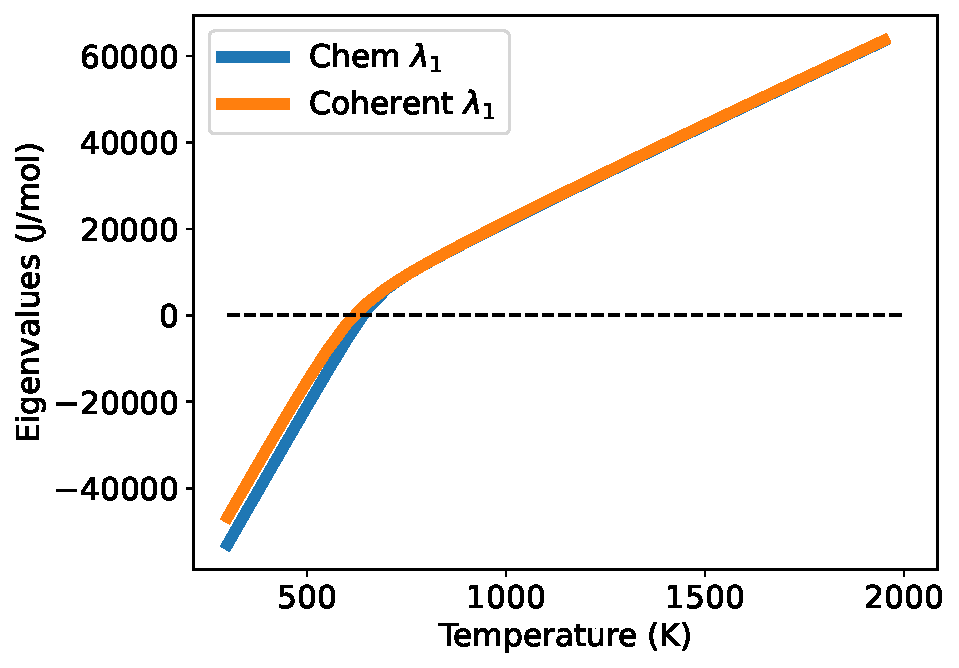
\includegraphics[width=.35\linewidth]{figs/eigenvalues_Hf1.pdf}}\hspace{.3 in}
         \subfloat[(b)]{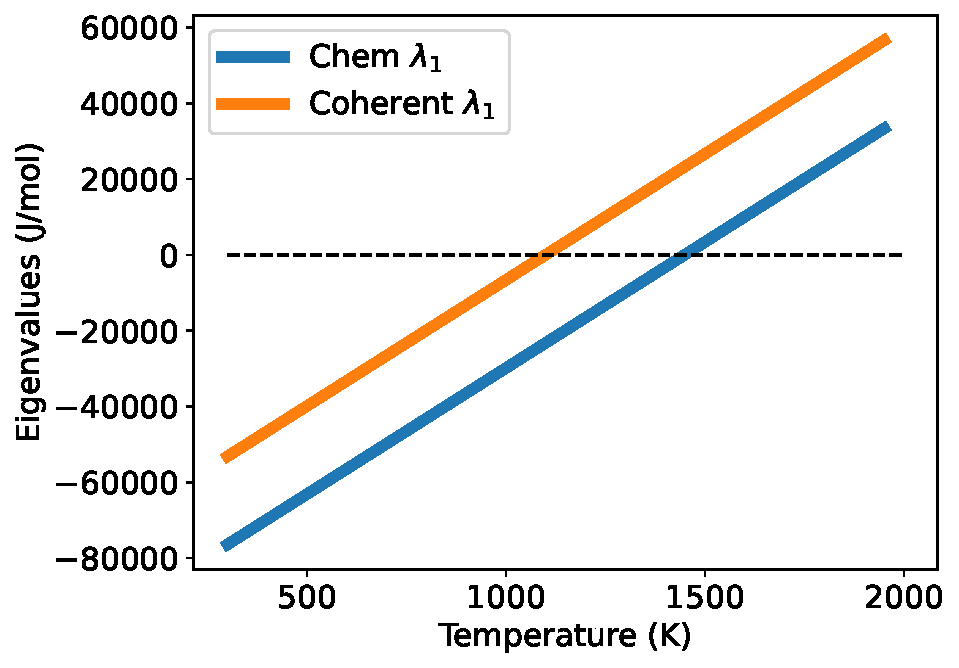
\includegraphics[width=.35\linewidth]{figs/eigenvalues_Hf25.pdf}}\\
         \subfloat[(c)]{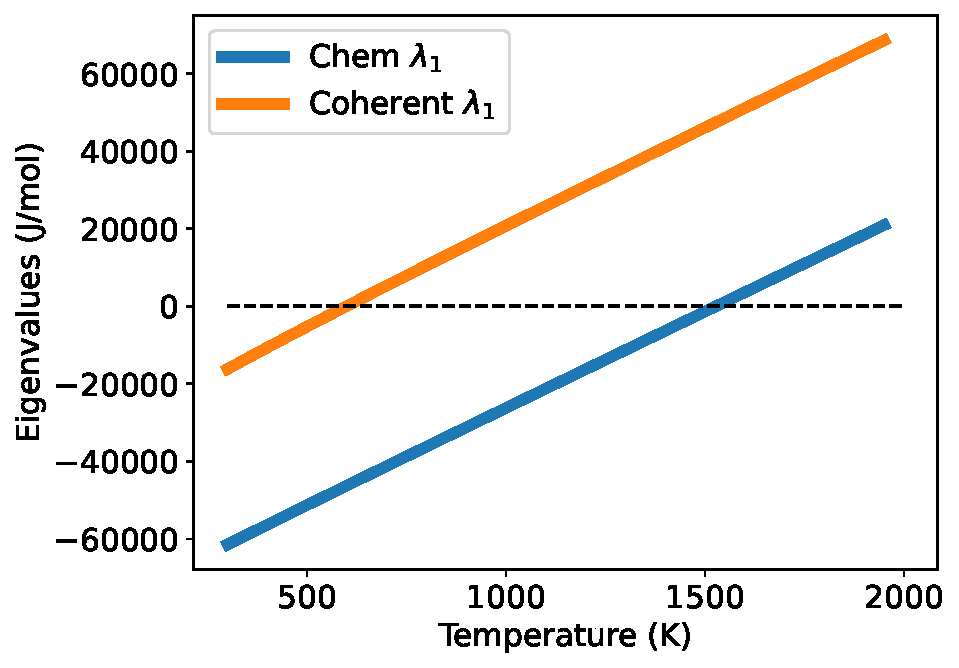
\includegraphics[width=.35\linewidth]{figs/eigenvalues_Hf4.pdf}}
         \caption{Gauge-invariant first eigenvalue of the chemical and coherent Gibbs energy Hessian as a function of temperature for BCC (a)~\ch{Hf_{0.10}Nb_{0.40}Ti_{0.40}V_{0.10}}, (b)~\ch{Hf_{0.25}Nb_{0.25}Ti_{0.25}V_{0.25}}, and (c)~\ch{Hf_{0.6}Nb_{0.1}Ti_{0.1}V_{0.2}}.
         Coherency shifts the spinodal temperature downward most strongly in Hf-rich alloys.
         The equiatomic composition (b) is coherently spinodal below ${\sim}\SI{800}{\kelvin}$, confirming \SI{500}{\celsius} as a tractable simulation temperature.}
\label{fig:eigenvalues}
\end{figure*}

\clearpage

\subsection{Binary Nb--V: First Demonstration of the MLIP-Informed Pipeline}
\label{sec:binary}

The binary Nb--V system is the first demonstration of the complete framework: a machine-learned interatomic potential (ORB) supplies the thermodynamic database, Jansson interpolation evaluates chemical potentials and their composition derivatives directly from the CALPHAD dataset --- bypassing finite-difference approximations --- and the spectral Cahn-Hilliard solver propagates the resulting elasto-chemical driving forces on the grid.
The single independent composition field isolates the Jansson derivative from multi-component complexity, and the well-characterized miscibility gap at \SI{500}{\celsius} with no spectator elements provides a clean validation setting before extension to the ternary and quaternary subsystems.
The equilibrium BCC\textsubscript{A2} tie-line endpoints at \SI{500}{\celsius} are an Nb-rich phase ($x_{\rm Nb} = 0.96$) and a V-rich phase ($x_{\rm Nb} = 0.36$), between which the stiffness tensors $C_{ij}$ and Vegard eigenstrain coefficient $\alpha_{\rm Nb} = \partial\ln a/\partial x_{\rm Nb}$ are linearly interpolated from SQS configurations evaluated with the ORB machine-learned interatomic potential.
The coefficient $\alpha_{\rm Nb} = 0.0874$ is evaluated at the tie-line midpoint ($x_{\rm Nb} = 0.66$, $a_{\rm ref} = \SI{3.228}{\angstrom}$), giving a total misfit strain $\varepsilon_T = -5.5\%$ between the two equilibrium phases and a molar volume $N_V = \SI{8.99e4}{\mol\per\metre\cubed}$.
Table~\ref{tab:binary_elastic} lists the full elastic constants and derived properties at both endpoints.

\begin{table}[!h]
    \centering
    \caption{%
        Elastic constants and Vegard eigenstrain parameters for the Nb--V
        BCC\textsubscript{A2} tie-line endpoints at \SI{500}{\celsius},
        computed from SQS configurations evaluated with the ORB
        machine-learned interatomic potential.
        $C' = (C_{11}-C_{12})/2$: tetragonal shear modulus;
        $A_Z = C_{44}/C'$: Zener anisotropy ratio;
        $\varepsilon_T = (a_{\rm ppt} - a_{\rm mat})/a_{\rm mat}$: misfit strain.
    }
    \label{tab:binary_elastic}
    \renewcommand{\arraystretch}{0.8}
    \setlength{\tabcolsep}{5pt}
    \begin{tabular}{lcc}
        \toprule
        Property & Nb-rich ($x_{\rm Nb}=0.96$) & V-rich ($x_{\rm Nb}=0.36$) \\
        \midrule
        \multicolumn{3}{l}{\textit{Composition and lattice parameter}} \\
        $x_{\rm Nb}$ & 0.96 & 0.36 \\
        $x_{\rm V}$  & 0.04 & 0.64 \\
        $a$ (\AA)    & 3.312 & 3.130 \\
        \midrule
        \multicolumn{3}{l}{\textit{Cubic elastic constants (GPa)}} \\
        $C_{11}$ & 243.6 & 259.3 \\
        $C_{12}$ & 119.7 & 145.0 \\
        $C_{44}$ &  20.6 &  18.0 \\
        $C' = (C_{11}-C_{12})/2$ & 62.0 & 57.2 \\
        \midrule
        \multicolumn{3}{l}{\textit{Derived elastic properties}} \\
        $G_{\rm VRH}$ (GPa) & 32.5 & 29.2 \\
        $B_{\rm VRH}$ (GPa) & 161.0 & 183.1 \\
        Poisson ratio $\nu$ & 0.406 & 0.424 \\
        Zener ratio $A_Z = C_{44}/C'$ & \textbf{0.332} & \textbf{0.315} \\
        \midrule
        \multicolumn{3}{l}{\textit{Vegard eigenstrain parameters (shared)}} \\
        $a_{\rm ref}$ (\AA) & \multicolumn{2}{c}{3.228} \\
        $\alpha_{\rm Nb} = \partial\ln a/\partial x_{\rm Nb}$ & \multicolumn{2}{c}{0.0874} \\
        $\varepsilon_T = \Delta a / a_{\rm mat}$ & \multicolumn{2}{c}{$-5.5\%$} \\
        $N_V$ (mol\,m$^{-3}$) & \multicolumn{2}{c}{$8.99\times10^{4}$} \\
        \bottomrule
    \end{tabular}
\end{table}

Both endpoints have $A_Z < 1$ (\Cref{tab:binary_elastic}), identifying $\langle 110 \rangle$ as the elastically soft direction.
Figure~\ref{fig:chem_vs_elastic} shows the output of the MLIP-informed pipeline across four mean compositions.
The chemical-only simulations (top row) produce isotropic interconnected domains at all four compositions, with no preferred orientation.
The elasto-chemical simulations (bottom row) reveal a composition-dependent response that is absent in the chemical-only case.
At $x_{\rm Nb}^0 = 0.50$, coherency strain completely suppresses spinodal decomposition and the field remains uniform, consistent with the coherent Hessian analysis showing that elastic energy closes the miscibility gap at the symmetric composition.
At $x_{\rm Nb}^0 = 0.60$ and $0.70$, decomposition proceeds and produces a labyrinthine, bicontinuous morphology with channels preferentially aligned along $\langle 110 \rangle$, reflecting the elastically soft direction ($A_Z < 1$).
At $x_{\rm Nb}^0 = 0.80$, the V-rich phase constitutes a small minority and forms isolated $\langle 110 \rangle$-elongated islands embedded in a continuous Nb-rich matrix.

The absence of decomposition at $x_{\rm Nb}^0 = 0.50$ reflects a direct thermodynamic consequence of coherency: at this composition and temperature, the elastic penalty is sufficient to render the smallest positive eigenvalue of the coherent Gibbs energy Hessian positive, stabilizing the alloy against all composition fluctuations. That the chemical-only simulation at the same composition decomposes freely establishes that this stability is entirely elastic in origin. Coherency strain thus closes the miscibility gap at the symmetric composition in Nb--V --- an effect that a purely chemical phase-field model would miss entirely.

\begin{figure}[!h]
    \centering
    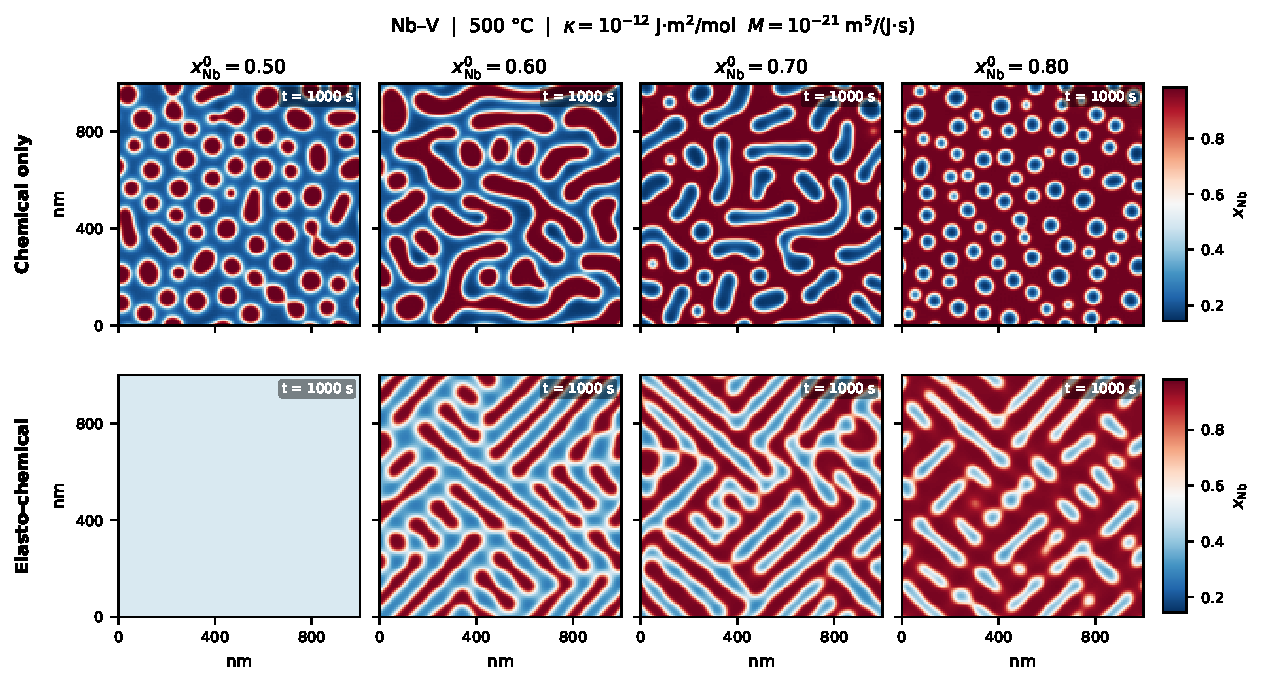
\includegraphics[width=\textwidth]{figs/chem_vs_elastic_final.pdf}
    \caption{%
        Simulated $x_{\rm Nb}$ microstructures from Cahn-Hilliard
        simulations of binary Nb--V BCC\textsubscript{A2} at
        \SI{500}{\celsius} ($128\times128$ grid,
        $L = \SI{1}{\micro\metre}$,
        $\kappa = \SI{1e-12}{\joule\metre\squared\per\mol}$,
        $M = \SI{5e-21}{\metre\tothe{5}\per\joule\per\second}$).
        Top row: chemical only.
        Bottom row: elasto-chemical (tensorial Vegard coupling,
        $\alpha_{\rm Nb} = 0.087$, cubic stiffness from SQS/DFT).
        Columns correspond to mean compositions
        $x_{\rm Nb}^0 = 0.50,\,0.60,\,0.70,\,0.80$.
        Colormap: $x_{\rm Nb}$ increases from blue (low) to red (high).
        Both phases have $A_Z < 1$, selecting $\langle 110 \rangle$-aligned
        boundaries and the characteristic diamond-faceted morphology in the
        elasto-chemical case.
    }
    \label{fig:chem_vs_elastic}
\end{figure}

\subsection{Ternary Nb--Hf--V: Temperature and Composition Dependence}
\label{sec:ternary}

Adding Hf to the binary Nb--V system changes the character of the spinodal instability qualitatively.
Table~\ref{tab:spinodal_regimes} summarizes four distinct regimes for the ternary Nb$_{50}$Hf$_5$V$_{45}$ alloy across \SIrange{500}{1000}{\celsius}, identified from the signs of the diagonal Hessian elements $H_{\rm Nb}$, $H_{\rm Hf}$, and $H_{\rm V} = H_{\rm Nb} + H_{\rm Hf} + 2H_{\rm Nb,Hf}$.
Above \SI{700}{\celsius}, no diagonal instability exists; the spinodal is driven solely by weak off-diagonal Nb--Hf coupling ($\lambda_{\min} \lesssim 0$) and produces no significant decomposition.
Between \SI{600}{\celsius} and \SI{700}{\celsius}, only $H_{\rm Nb} < 0$: Nb segregates asymmetrically against a stable V$+$Hf background, with Hf acting as an inert spectator.
Below \SI{500}{\celsius}, $H_{\rm V}$ also turns negative, recovering a binary-like Nb--V demixing, but Hf remains a positive-curvature stiffener that suppresses $\Delta t$.
The most numerically tractable temperature for this ternary is \SI{700}{\celsius}, where the Nb-driven spinodal ($|\lambda_{\min}| = \SI{13272}{\joule\per\mol}$) is active without the stiffness penalty, albeit with a driving force approximately six times weaker than at \SI{500}{\celsius}.

\begin{table}[!h]
    \centering
    \caption{%
        Spinodal character and equilibrium two-phase compositions as a function
        of temperature for the binary Nb$_{50}$V$_{50}$ and ternary
        Nb$_{50}$Hf$_5$V$_{45}$ BCC\textsubscript{A2} alloys.
        Signs of the diagonal Hessian elements indicate whether each element
        is individually unstable ($H_{ii} < 0$, driving force) or stable
        ($H_{ii} > 0$, spectator).
        $H_{\rm V}$ is derived via
        $H_{\rm V} = H_{\rm Nb} + H_{\rm Hf} + 2H_{\rm Nb,Hf}$.
    }
    \label{tab:spinodal_regimes}
    \scriptsize
    \renewcommand{\arraystretch}{1.0}
    \begin{tabularx}{\textwidth}{lllll}
        \toprule
        Regime & System & Diagonal instabilities & Physical character & Equilibrium BCC phases$^{a}$ \\
        \midrule
        $T < \SI{750}{\celsius}$
            & Binary Nb$_{50}$V$_{50}$
            & $H_{\rm Nb} = H_{\rm V} < 0$
            & Symmetric Nb$\leftrightarrow$V demixing; both components drive decomposition equally
            & BCC$_1$: Nb$_{99}$V$_{1}$\newline BCC$_2$: Nb$_{1}$V$_{99}$ \\
        $T > \SI{700}{\celsius}$
            & Ternary Nb$_{50}$Hf$_5$V$_{45}$
            & None ($H_{\rm Nb},\,H_{\rm Hf},\,H_{\rm V} > 0$)
            & No diagonal instability; only weak off-diagonal Nb--Hf coupling drives marginal spinodal ($\lambda_{\min} \lesssim 0$); no significant decomposition
            & Single-phase BCC: Nb$_{50}$Hf$_{5}$V$_{45}$ \\
        \SIrange{600}{700}{\celsius}
            & Ternary Nb$_{50}$Hf$_5$V$_{45}$
            & $H_{\rm Nb} < 0$ only
            & Asymmetric spinodal: Nb segregates against a stable V$+$Hf matrix; Hf acts as inert spectator
            & BCC$_1$: Nb$_{90}$Hf$_{9}$V$_{1}$\newline BCC$_2$: Nb$_{2}$Hf$_{0.1}$V$_{98}$ \\
        $T < \SI{500}{\celsius}$
            & Ternary Nb$_{50}$Hf$_5$V$_{45}$
            & $H_{\rm Nb} < 0$,\; $H_{\rm V} < 0$
            & Binary-like Nb--V demixing; Hf remains stable ($H_{\rm Hf} > 0$) and imposes numerical stiffness
            & BCC$_1$: Nb$_{91}$Hf$_{9}$V$_{0.3}$\newline BCC$_2$: Nb$_{0.6}$Hf$_{0.04}$V$_{99}$ \\
        \bottomrule
        \multicolumn{5}{l}{\footnotesize $^{a}$~Equilibrium tie-line endpoints computed with \texttt{pycalphad}
            (\texttt{BCC\_A2} miscibility gap) using an ORB-MLIP CALPHAD database for the HfNbTiV system.
            Subscripts are at.\%; representative temperatures: \SI{500}{\celsius} for
            $T<\SI{750}{\celsius}$ rows, \SI{700}{\celsius} for the
            \SIrange{600}{700}{\celsius} row.}
    \end{tabularx}
\end{table}

Figure~\ref{fig:ternary_summary} consolidates three further perspectives on the ternary system.
The Hf sweep (panels a--e) shows that at low Hf fractions ($x_{\rm Hf}^0 = 0.05$, 0.10) decomposition produces isolated Nb-rich precipitates consistent with a minority-phase microstructure; increasing Hf to 0.20 and 0.25 shifts the tie-line endpoints and produces well-developed bicontinuous Nb--V domains, indicating that Hf progressively deepens the miscibility gap.
The middle row (panels e--f) isolates the elastic contribution at $x_{\rm Hf}^0 = 0.25$: the chemical-only simulation (e) produces isotropic interconnected domains, while the elasto-chemical case (f) remains nearly uniform, demonstrating that coherency strain again closes the miscibility gap at this composition, extending the suppression seen in the binary at $x_{\rm Nb}^0 = 0.50$ to the ternary.
The bottom row (panels g--h) shows the temperature dependence for Nb$_{50}$Hf$_5$V$_{45}$: at \SI{500}{\celsius} (g) decomposition is early-stage with small, diffuse Nb-rich clusters, while at \SI{600}{\celsius} (h) the domains are better developed despite the higher temperature, consistent with the Hessian analysis showing that $H_{\rm Nb} < 0$ with a moderate driving force at \SI{600}{\celsius} while the system sits closer to the spinodal boundary at \SI{500}{\celsius} for this dilute-Hf composition.
Panel (i) places these simulations in context by showing the ternary BCC\textsubscript{A2} miscibility gap across all three binary subsystems (Hf--Nb, Nb--V, Hf--V), with the composition space accessible to the ternary highlighted.

\begin{figure*}[!h]
    \centering
    \begin{overpic}[width=\textwidth]{figs/hf_sweep}
    \put(0, 20){\textbf{(a)}}
    \end{overpic}
    %%%
    \begin{overpic}[width=\textwidth]{figs/hf_sweep_elastic}
    \put(0, 20){\textbf{(b)}}
    \end{overpic}
    %%%
    \begin{overpic}[width=0.6\textwidth]{figs/Spinodal Ternary Phase Diagram Figure.png}
    \put(0, 80){\textbf{(c)}}
    \end{overpic}
    \caption{%
        Hf-content sweep of $x_{\rm Nb}$ microstructures in ternary
        Nb--Hf--V BCC\textsubscript{A2} at \SI{500}{\celsius}
        ($128\times128$ grid, $L = \SI{1}{\micro\metre}$,
        $\kappa = \SI{1e-12}{\joule\metre\squared\per\mol}$,
        $M_{\rm Nb} = \SI{5e-21}{\metre\tothe{5}\per\joule\per\second}$).
        \textbf{(a)} Chemical-only simulations.
        \textbf{(b)} Elasto-chemical simulations with Vegard coherency strain;
        panels marked ``simulation pending'' are reserved for calculations in
        progress.
        \textbf{(c)} Ternary BCC\textsubscript{A2} miscibility gap across all
        three binary subsystems (Hf--Nb, Nb--V, Hf--V).
        Colormap: $x_{\rm Nb}$ increases from blue (low) to red (high).
    }
    \label{fig:ternary_summary}
\end{figure*}

\subsection{Quaternary HfNbTiV: Phase-Field Prediction and Experimental Validation}
\label{sec:quaternary}

\subsubsection{Chemical-only microstructure and CALPHAD tie-line}

The equiatomic composition Nb$_{25}$Hf$_{25}$Ti$_{25}$V$_{25}$ satisfies both criteria identified in Section~\ref{sec:stability_landscape}: $\lambda_{\min} < 0$ at \SI{500}{\celsius} and, with the mobility assignments described below, sufficient microstructural evolution is accessible within $10^6$ steps.
Figure~\ref{fig:quaternary_chem} shows the composition fields from a chemical-only Cahn-Hilliard simulation ($128\times128$ grid, $L = \SI{1}{\micro\metre}$, $\Delta t = \SI{0.1}{\second}$, $\boldsymbol{\kappa} = [\num{1e-12},\,\num{7e-12},\,\num{1e-12}]\,\si{\joule\metre\squared\per\mol}$, $\mathbf{M} = \operatorname{diag}[\num{5e-21},\,\num{5e-23},\,\num{5e-21}]\,\si{\metre\tothe{5}\per\joule\per\second}$) at step 600{,}000.
Ellipsoidal V-rich precipitates form in an Nb/Hf/Ti-rich matrix; the diffuse Hf halos around precipitate cores reflect the tenfold lower Hf mobility relative to Nb and Ti rather than an independent Hf instability.

To validate the partitioning directions and obtain physically correct tie-line endpoints for the elasto-chemical simulation, we computed the CALPHAD equilibrium tie-line at \SI{500}{\celsius} using \texttt{pycalphad} with an ORB-MLIP CALPHAD database for the HfNbTiV system (\Cref{tab:quaternary_tieline}).
Two BCC\textsubscript{A2} phases coexist: an Nb/Hf/Ti-rich matrix (phase fraction $\approx 0.67$) and a V-rich precipitate (phase fraction $\approx 0.33$).
The phase-field partitioning directions match the CALPHAD prediction for all four elements; Nb and V compositions agree quantitatively, while Hf and Ti have not yet reached their equilibrium values at step 600{,}000, consistent with slow Hf kinetics and residual V in the matrix.

\begin{table}[!h]
    \centering
    \caption{%
        CALPHAD equilibrium tie-line endpoints for equiatomic
        Nb$_{25}$Hf$_{25}$Ti$_{25}$V$_{25}$ BCC\textsubscript{A2} at
        \SI{500}{\celsius}, computed with \texttt{pycalphad} using the
        ORB-MLIP CALPHAD database for the HfNbTiV system.
        Phase-field composition ranges from the final frame (step 600{,}000)
        are shown for comparison; PFM values are non-equilibrium, particularly
        for Hf (slow kinetics) and V (matrix still draining).
    }
    \label{tab:quaternary_tieline}
    \renewcommand{\arraystretch}{1.3}
    \setlength{\tabcolsep}{5pt}
    \begin{tabular}{llcccc}
        \toprule
        & & $x_{\rm Nb}$ & $x_{\rm Hf}$ & $x_{\rm Ti}$ & $x_{\rm V}$ \\
        \midrule
        \multirow{2}{*}{CALPHAD tie-line}
            & Matrix ($f \approx 0.67$)
            & 0.300 & 0.371 & 0.305 & 0.024 \\
            & Precipitate ($f \approx 0.33$)
            & 0.148 & 0.002 & 0.136 & 0.714 \\
        \midrule
        \multirow{2}{*}{PFM (step 600{,}000)}
            & Matrix
            & $\approx 0.30$ & $\approx 0.33$ & $\approx 0.29$ & $\approx 0.11$ \\
            & Precipitate
            & $\approx 0.11$ & $\approx 0.06$ & $\approx 0.06$ & $\approx 0.68$ \\
        \bottomrule
    \end{tabular}
\end{table}

\begin{figure}[!h]
    \centering
    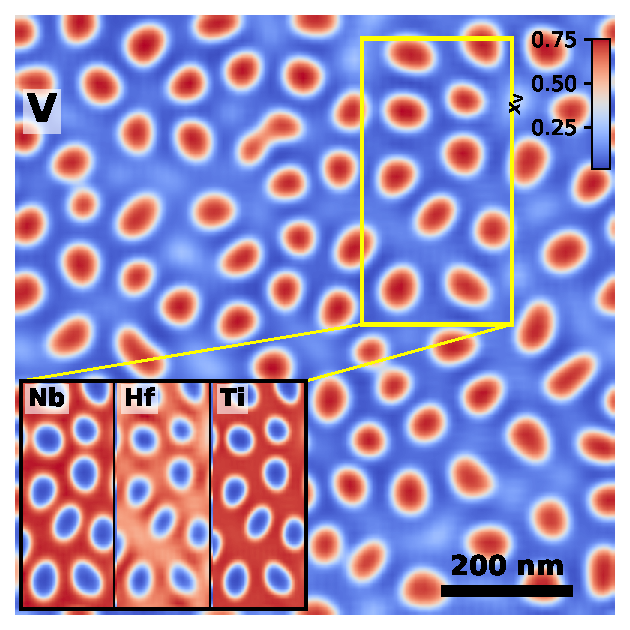
\includegraphics[width=\textwidth]{figs/quaternary_chem_step600k.pdf}
    \caption{%
        Composition fields from the chemical-only Cahn-Hilliard simulation of
        equiatomic Nb$_{25}$Hf$_{25}$Ti$_{25}$V$_{25}$ BCC\textsubscript{A2}
        at \SI{500}{\celsius} ($128\times128$ grid, $L = \SI{1}{\micro\metre}$,
        step 600{,}000, $\Delta t = \SI{0.1}{\second}$).
        From left to right: $x_{\rm Nb}$, $x_{\rm Hf}$, $x_{\rm Ti}$, $x_{\rm V}$.
        V-rich precipitates (blue in $x_{\rm Nb}$, $x_{\rm Hf}$, $x_{\rm Ti}$;
        red in $x_{\rm V}$) are embedded in an Nb/Hf/Ti-rich matrix.
        Diffuse halos in $x_{\rm Hf}$ reflect the tenfold lower Hf mobility
        ($M_{\rm Hf} = \SI{5e-23}{\metre\tothe{5}\per\joule\per\second}$).
        Partitioning directions are consistent with the CALPHAD tie-line
        (\Cref{tab:quaternary_tieline}).
    }
    \label{fig:quaternary_chem}
\end{figure}

\subsubsection{Elasto-chemical prediction and comparison with experiment}

The elastic response of the quaternary system differs fundamentally from the binary baseline of Section~\ref{sec:binary}.
At the CALPHAD tie-line matrix composition, the SQS/DFT interpolant yields $A_Z^{\rm mat} = 1.52 > 1$, identifying $\langle 100 \rangle$ as the elastically soft direction — the opposite selection from the binary NbV case ($A_Z = 0.33 < 1$).
Table~\ref{tab:elastic_comparison} compares the full set of model predictions against the experimental characterization of equiatomic HfNbTiV by An~et~al.\ \cite{an2021spinodal}, who identified two coexisting BCC\textsubscript{A2} phases in an as-cast alloy by XRD, HAADF-STEM, and EDS.

\begin{table}[!h]
    \centering
    \caption{%
        Predicted and experimentally measured properties for the equiatomic
        BCC\textsubscript{A2} HfNbTiV alloy.
        Experimental values are from An~et~al.\ \cite{an2021spinodal} (as-cast,
        characterized by XRD, HAADF-STEM, and EDS).
        Binary predictions use the NbV tie-line endpoints; quaternary
        predictions use the CALPHAD tie-line at \SI{500}{\celsius}
        (\Cref{tab:quaternary_tieline}).
        $A_Z = 2C_{44}/(C_{11}-C_{12})$: $A_Z > 1$ selects
        $\langle 100 \rangle$ modulation, $A_Z < 1$ selects
        $\langle 110 \rangle$.
        $\varepsilon_T = (a_{\rm ppt} - a_{\rm mat})/a_{\rm mat}$.
    }
    \label{tab:elastic_comparison}
    \renewcommand{\arraystretch}{1.3}
    \setlength{\tabcolsep}{4pt}
    \begin{tabularx}{\textwidth}{lXXX}
        \toprule
        Property
            & Experiment \cite{an2021spinodal}
            & Binary NbV (this work)
            & Quaternary NbHfTiV (this work) \\
        \midrule
        Precipitate enriched in
            & Hf $+$ V
            & V
            & V (Hf in matrix) \\
        Matrix enriched in
            & Nb $+$ Ti
            & Nb
            & Nb, Hf, Ti \\
        Precipitate phase fraction
            & $\approx 1/3$
            & ---
            & $\approx 0.33$ \\
        $a_{\rm mat}$ (\AA)
            & 3.313
            & 3.312
            & 3.382 \\
        $a_{\rm ppt}$ (\AA)
            & 3.259
            & 3.130
            & 3.089 \\
        $\varepsilon_T$
            & $-1.6\%$ (XRD); $0.54\%$ (TEM)
            & $-5.5\%$
            & $-8.7\%$ \\
        $A_Z$ (matrix)
            & ---
            & 0.33
            & \textbf{1.52} \\
        $A_Z$ (precipitate)
            & ---
            & 0.31
            & 0.32 \\
        Spinodal modulation direction
            & $\langle 100 \rangle$
            & $\langle 110 \rangle$ (predicted)
            & $\langle 100 \rangle$ (predicted) \\
        Modulation wavelength
            & ${\approx}\SI{50}{\nano\metre}$
            & ---
            & ${\approx}50$--\SI{100}{\nano\metre} \\
        \bottomrule
    \end{tabularx}
\end{table}

Three findings emerge from this comparison.

\textit{Hf partitioning is inconsistent between the CALPHAD model and experiment.}
An~et~al.\ demonstrate via HAADF-STEM Z-contrast that Hf ($Z = 72$, the heaviest constituent) enriches the precipitate phase ($\beta^*$), co-segregating with V.
The ORB-MLIP CALPHAD model assigns Hf to the matrix alongside Nb and Ti (\Cref{tab:quaternary_tieline}).
The most likely origin of this discrepancy is the thermal history: the experimental alloy was drop-cast and spinodal decomposition occurred during rapid cooling from the melt, far from the \SI{500}{\celsius} equilibrium tie-line used in the simulation.
Non-equilibrium partitioning during rapid quenching can favor kinetically accessible configurations that differ from the thermodynamic ground state, particularly for a heavy element such as Hf whose equilibrium diffusivity is low.

\textit{The misfit strain is overestimated by the CALPHAD model.}
An~et~al.\ report a lattice misfit of $-1.6\%$ from XRD peak separation and $0.54\%$ from TEM atomic-column measurements, both substantially smaller than the $-8.7\%$ predicted by the quaternary CALPHAD tie-line.
This overestimate is a direct consequence of the incorrect Hf partitioning: if Hf (large atomic radius, $a_{\rm Hf}^{\rm BCC} \approx \SI{3.62}{\angstrom}$) were to co-enrich the precipitate with V (small atomic radius, $a_{\rm V}^{\rm BCC} \approx \SI{3.03}{\angstrom}$), the opposing contributions to the precipitate lattice parameter would partially cancel, yielding a much smaller net misfit consistent with experiment.
The binary NbV misfit of $-5.5\%$ is also larger than the experimental value, though less severely so.

\textit{The quaternary elastic anisotropy correctly predicts the observed spinodal modulation direction.}
The HAADF-STEM fast Fourier transform patterns in An~et~al.\ (Fig.~1(e,f) of that work) show spinodal modulation wavevectors along $\langle 100 \rangle$, the elastically soft direction for alloys with $A_Z > 1$.
The quaternary CALPHAD model gives $A_Z^{\rm mat} = 1.52 > 1$ for the Nb/Hf/Ti-rich matrix, correctly selecting $\langle 100 \rangle$ as the preferred modulation direction.
The binary NbV model gives $A_Z = 0.33 < 1$ for both phases, which would predict $\langle 110 \rangle$ modulation, inconsistent with the experimental observation.
This agreement demonstrates that the multi-element matrix composition, rather than the V-rich precipitate, controls the elastic anisotropy and hence the morphological selection in this system.
The phase fraction ($\approx 1/3$) and modulation wavelength (${\approx}50$--\SI{100}{\nano\metre}) are also reproduced by the quaternary model.

\section{Conclusions and Future Work}

In this work, we demonstrated an open-source workflow for high-throughput microstructure stability analysis. Firstly, if a suitable CALPHAD model is not available to the modeler, it can be created through PhaseForge. The chemical Hessian is then determined analytically and efficiently via Jansson derivatives. Coherent strain contributions can be added through an analytically differentiable bond model and MLIP estimates for elastic constants. Lastly, following a clever change of basis, gauge-invariant eigenvalues and eigenvectors of the chemical and coherent spinodal can be investigated at specific compositions as functions of temperature or visualized at a given temperature over a high-dimensional composition space through affine projections. This workflow provides many valuable extensions to the foundational stability analysis framework produced by Koneru, Kadirvel, and Wang \cite{koneru2022high}, to include 1) open-source access, 2) whitebox CALPHAD model knowledge, 3) improved efficiency and robustness of Gibbs energy derivatives, 4) modeling coherent strain contributions, and 5) visualization in large composition spaces via one two-dimensional plot.

However, there are still plenty of future directions to further extend this workflow. A model for homogeneous elastic Gibbs energy contributions could be incorporated in addition to contributions from coherent strain due to composition fluctuations. MLIPs could also be used to create bond models for other crystal structures, and coherent strain elastic contributions could be modeled for materials that do not behave isotropically. Lastly, implementation of second-order Jansson derivatives would provide analytic calculation of third-order derivatives of the Gibbs energy with respect to composition, enabling the analytic calculation of critical points.

\section*{Code Availability}

The thermodynamic databases used in this work were generated using PhaseForge~\cite{phaseforge2025} (\url{https://github.com/dogusariturk/PhaseForge}). The CALPHAD-coupled phase-field solver, spinodal stability analysis workflow, and all simulation configs and post-processing scripts are openly available at \url{https://github.com/vahid2364/PhaseFoundry}. Elastic constants were computed from SQS configurations evaluated with the ORB-v2 machine-learned interatomic potential (\url{https://github.com/orbital-materials/orb-models}) and the GRACE-2L potential; both are publicly available from their respective developers.

\section*{Acknowledgments}
 RA also wishes to acknowledge the support from NSF through Grant No. NSF-DMREF-2119103. R.A.~and D.S.~acknowledge support from the Army Research Office (ARO) through Grant No.~W911NF-22-2-0117. Portions of this research were conducted with the advanced computing resources provided by Texas A\&M High Performance Research Computing.
 

\bibliographystyle{elsarticle-num}
\biboptions{numbers,sort&compress}
\bibliography{refs}

\end{document}
